\section[Experimental Study]{Experimental Study\protect\footnote{Reproducibility package: https://github.com/anonymous-author-1000/auto-peira/}}\label{sec:study}

\subsection{Motivation and Goals}

The Peira process is based on recruiting, training, and having experimental participants perform rating tasks. This entails cost and effort for those involved. With the advent of Large Language Models (LLMs) \cite{LLM.survey} the question of whether such models can act as more accessible and cost-effective proxies for human input becomes relevant. At the same time, as increased LLM size is known to improve capability but also increase computational cost and environmental impact, it is also useful to know how small an LLM can be and still play the role of a faithful substitute for human participants. The experimental study we report below addresses these research goals. The specific research questions (RQs) are:

\textbf{RQ1.} Can LLMs be used as substitutes for human raters in Peira?

\textbf{RQ2.} Does model size affect the performance of LLMs in executing Peira's rating tasks?

To answer these questions, we apply Peira on a chosen modeling language in two ways: (a) with human participants performing the ratings, as proposed by the method, and (b) with LLMs performing the ratings instead. To assess whether LLMs perform at human level so as to justify their use as substitutes for human raters (RQ1), we measure and compare the rating performance, in terms of precision and recall with respect to the authoritative ratings, of LLMs vs. humans. For LLMs to be considered an appropriate substitute for humans for the task, we require that their performance falls within a confidence interval of average human performance; otherwise, if LLMs perform significantly better or worse than humans, they cannot be considered faithful proxies of human judgment for this task. Furthermore, the LLMs are sampled to be of different sizes with respect to their number of parameters in order to allow size to be investigated as a predictor of performance in the classification tasks (RQ2).

\subsection{Study Design}

\subsubsection{Language}

For our study we choose a language recently introduced in the literature for modeling reinforcement learning domains \cite{LKMG.24}. The language, called iStar-DT, is an extension of iStar 2.0 \cite{DaFH.16}, a language for intentional modeling of socio-technical systems. The original iStar 2.0 includes entities (unary concepts) such as \textit{actors}, which are participants in the socio-technical system in question, \textit{goals} adopted and pursued by said actors, \textit{tasks}, which describe specific actions performed by actors to pursue their goals, and \textit{qualities}, which describe attributes that actors want to be satisfied while attaining goals. Relationships include \textit{AND-} and \textit{OR-decompositions} of goals into subgoals and tasks, and  \textit{contribution links} that show how satisfaction of goals, tasks, or qualities affect satisfaction of other qualities. 

The iStar-DT extension adds concepts for modeling the state of the environment in which actors pursue their goals as well as to express temporal constraints in task execution and goal satisfaction. Thus, \textit{affects} relationships connect tasks with \textit{effect} elements showing how tasks affect the state of the environment, and \textit{precedes} relationships express that performance of a task requires prior performance or satisfaction of another task or goal.  The extension also introduces \textit{pre-effect} and \textit{pre-quality} elements to represent the state of effects and qualities at a specified previous time. A visual notation is also proposed to diagrammatically signify these concepts.

The details of iStar-DT are beyond the scope of this presentation; readers can refer to the publication introducing it \cite{LKMG.24}. Interestingly, the authors' most recent publication \cite{LDKM+26} features updates and simplifications to the iStar-DT ontology. In this study, we adopt their original proposal \cite{LKMG.24}, without harming our research strategy. Overall, the vocabulary $V$ under investigation includes 18 elements, 9 of which are entities (unary concepts, e.g. ``goal'', ``task'', etc.) and the remaining 9 are relationships (binary concepts, e.g., ``affects'', ``positively contributes to'', etc.). 

\subsubsection{Instrument and Tasks for Human Participants}

With the language under investigation selected, we next develop the rating acquisition instrument, according to the Peira specifications. The instrument is administered online and consists of a sequence of screens in which participants perform various tasks as follows. A video welcoming participants and outlining the engagement is first presented, followed by a 15 minute video presentation of iStar-DT. This, in turn, is followed by a screen with video comprehension exercises, to be used for filtering inattentive participants. Next, participants are given a list of selected pairs of iStar-DT's entities and relationships and asked to rate the conceptual overlap of the pairs. The screen that follows is the heart of the instrument: the participants are shown a video describing one of two case descriptions. The two cases considered are inspired by the two examples offered in the iStar-DT publications \cite{LKMG.24,LDKM+26}, namely a temperature controller and an engine manufacturer. The video simply walks participants through the text of the case. Below the video, a series of elements to be classified by an entity is presented (e.g., \textit{``Have Engine Assembled''}, \textit{``Parts Acquired in Time''}, \textit{``Engine Manufacturer''}), below each of which, a multiple-choice inventory of the nine entities of $V$ (e.g., ``actor'', ``goal'', etc.) plus the ``None'' option are displayed. Participants are asked to check one or more of the items in the inventory if they believe that the element should be modeled using the corresponding term. Below the elements for entity classification is, likewise, a list of tuples (e.g., \textit{``Parts Never Acquired \_\_\_\_ Order is Cancelled''} and \textit{``Construction is of Bad Quality \_\_\_\_ Reputation''}) to be classified under one of the relationships (e.g., \textit{``deterministically affects''}, \textit{``negatively contributes''}) listed, again, as a multiple-choice inventory. The final screen, prior to acquisition of demographic information and feedback on the instrument, asks participants to self-report their perception of the completeness of the vocabulary. Psytoolkit is used for constructing and administering the instruments \cite{Stoe.10,Stoe.17}. Participants are expected to dedicate 45' of their time to complete the tasks. Example screenshots of the instrument are offered in our reproducibility package \cite{TR}. 

\subsubsection{Instrument and Tasks for LLM Participants}
Rather than an on-line sequence of screens, LLMs are offered a prompt with equivalent content. The prompt begins with a transcription of the video presentation of the language, followed by a reproduction of the content of the subsequent screens, including the cases (again, transcribed), the elements, and the options. Directions are added on how the LLMs are supposed to render a response in the form of a JSON specification, for us to then convert into R dataframes for the analysis using the Peira toolset. A single long prompt is submitted and the LLM response to that prompt is utilized. When the LLM provided obviously invalid output (e.g., syntactically erroneous or empty JSON), which occasionally happened -- more below -- we followed up with short requests to the LLM to reproduce the outptout correcting those mistakes. Note also that while human participants are assigned to one of the two cases, the LLM prompt includes both cases. The prompt is 36,250 characters, so an approximate 9K-11K tokens, depending on model, according to literature \cite{VHSB+24} and OpenAI's estimation tool \cite{OpenAI.tokenizer}.

\subsubsection{Human Participant Sampling}
Human participation was sought from the online participants of Prolific \cite{Prol.26}. They are screened for having an undergraduate bachelors (BA/BSc/other) or technical/community college degree in Information and Communication Technology. A total of forty (40) participants are invited and each case was randomly assigned twenty (20) of them.

\subsubsection{LLM Participant Sampling}
A total of nineteen (19) LLMs were sampled from the OpenRouter \cite{openRouter} platform, selected to represent a broad range of model sizes, architectural families, and developers. The sample spans from 1B to 480B total parameters, covering small (1B–12B), medium (14B–49B), large (70B–120B), and very large (198B–480B) models --- see Table \ref{tab:llm_list}. The selection includes general-purpose models alongside more specialized variants, such as a code-focused model (\textit{qwen/qwen3-coder}) and a reasoning-oriented model (\textit{arcee-ai/trinity-large-thinking}). Context window lengths are all 128K tokens except: \textit{microsoft/phi-4} (16K), \textit{qwen/qwen3-coder} (1M), and \textit{stepfun/step-3.7-flash} (256K). 


\begin{table}[t]
\centering
\caption{\label{tab:llm_list}List of LLMs used for the study. Size in Billions of parameters. For Mixture of Experts (MoE) \cite{SMMD+17} architectures, total available parameters are displayed.}
\centering
\fontsize{8}{10}\selectfont
\begin{tabular}[t]{rlr}
\toprule
ID & Model & Size\\
\midrule
1 & qwen/qwen3-coder & 480\\
2 & nousresearch/hermes-4-405b & 405\\
3 & stepfun/step-3.7-flash & 198\\
4 & openai/gpt-oss-120b & 120\\
5 & nvidia/nemotron-3-super-120b-a12b & 120\\
\addlinespace
6 & qwen/qwen3-next-80b-a3b-instruct & 80\\
7 & qwen/qwen-2.5-72b-instruct & 72\\
8 & arcee-ai/trinity-large-thinking & 70\\
9 & meta-llama/llama-3.3-70b-instruct & 70\\
10 & nvidia/llama-3.3-nemotron-super-49b-v1.5 & 49\\
\addlinespace
11 & mistralai/mistral-small-2603 & 24\\
12 & openai/gpt-oss-20b & 20\\
13 & microsoft/phi-4 & 14\\
14 & google/gemma-3-12b-it & 12\\
15 & nvidia/nemotron-nano-9b-v2 & 9\\
\addlinespace
16 & arcee-ai/trinity-mini & 8\\
17 & qwen/qwen3-8b & 8\\
18 & google/gemma-3-4b-it & 4\\
19 & meta-llama/llama-3.2-1b-instruct & 1\\
\bottomrule
\end{tabular}
\end{table}

\subsubsection{Hypotheses and Planned Analysis}

\begin{figure}[th]
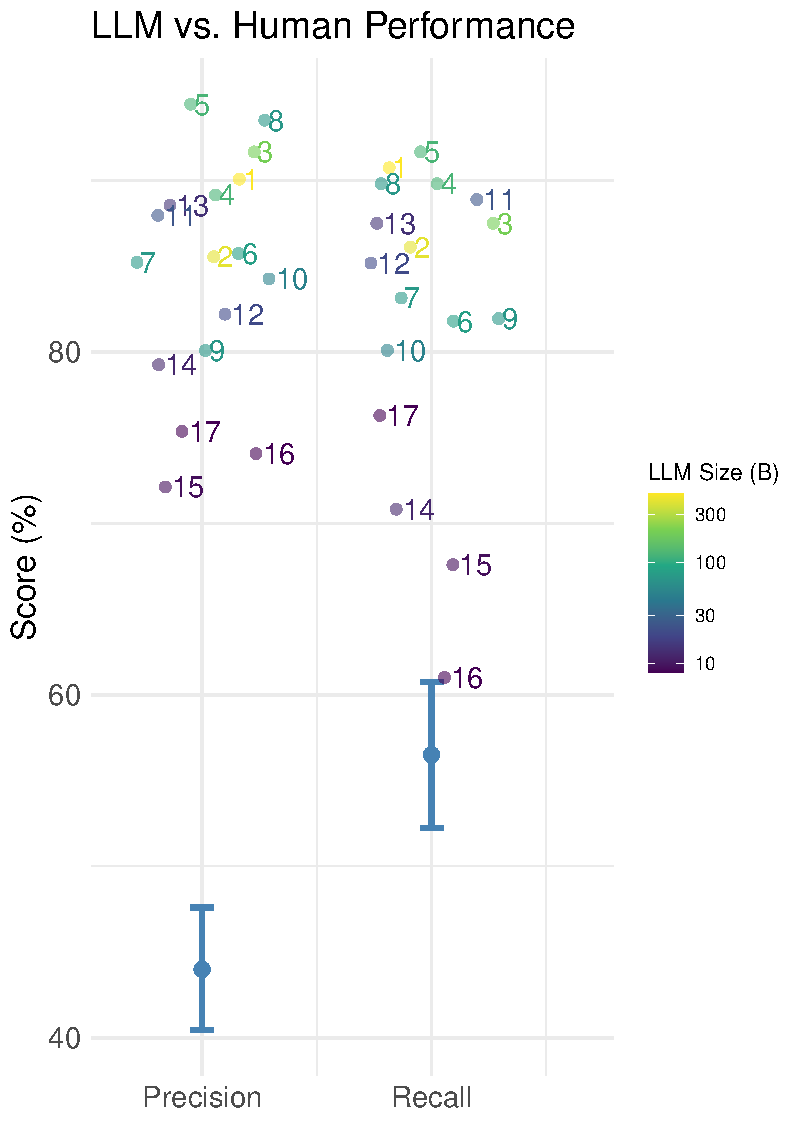
\includegraphics[width=0.8\columnwidth]{img/iRL-fig-ci.plot.pdf} 
\caption{95\% confidence interval of mean human performance and performance data of individual LLMs (dots).}\label{fig:ci}
\end{figure}


In accordance with our research questions, the null hypotheses (whose rejection is attempted) are as follows:

\textbf{H$_0^1$.} For each LLM, performance falls within the 95\% confidence interval of the average human performance, measured in terms of per-participant precision and recall --- $\mathrm{prec}^{pp}_V(p)$ and $\mathrm{rec}^{pp}_V(p)$.

\textbf{H$_0^2$.} Model size does not have a relationship with performance in terms of, again accuracy. 

To attempt to reject H$_0^1$, we form the corresponding confidence interval and check if the precision and recall of each LLM falls within the interval. To reject H$_0^2$ we perform a simple regression using model size as predictor and the F1 score (harmonic mean of precision and recall) as response variable. 

\subsection{Results}

\begin{table}
\centering
\caption{\label{tab:dems}Participant Counts and Ages by Sex and Case.}
\centering
\begin{tabular}[t]{llrr}
\toprule
Case & Sex & Average Age & Count\\
\midrule
 & Female & 33 & 8\\

\multirow{-2}{*}{\raggedright\arraybackslash Manufacturing} & Male & 34 & 12\\
\cmidrule{1-4}
 & Female & 32 & 5\\

\multirow{-2}{*}{\raggedright\arraybackslash Thermostat} & Male & 30 & 10\\
\bottomrule
\end{tabular}
\end{table}

\subsubsection{Participation}

Of the forty (40) participants invited, five (5) disqualified due to a low score in the video comprehensibility questions. This resulted in a total of thirty-five (35) usable cases. The statistics in terms of case they worked on, sex, and age can be found in Table \ref{tab:dems}. Of the 19 LLMs, all but two small ones (\textit{meta-llama/llama-3.2-1b-instruct} and \textit{google/gemma-3-4b-it}) gave usable output resulting in 17 performance data points in total.



\subsubsection{Outcome}

The LLMs achieved higher performance than humans overall. Table \ref{tab:medians} shows the median precision and recall values for Humans and LLMs, accounted per concept and per participant. Furthermore, we consider the 35 data human points and create studentized bootstrap confidence intervals for precision and recall (bootstrap-t method; R = 999 iterations) at the 95\% confidence level. The intervals can be viewed in Figure \ref{fig:ci} along with labeled dots representing the corresponding performance of each LLM. All LLM points fall outside the 95\% confidence interval, meaning that for each LLM, we reject the null hypothesis \textbf{H$_0^1$} that its precision and recall are equal to the human population mean ($\alpha$ = 0.05). Thus, by the standard that we set above for justifying  substitutability of humans by LLMs, none of the LLMs can play that specific role: they are too well-performing to be representative of human performance. An alternative visualization can be viewed in Figure \ref{fig:scatter}, where the performance of individual human and LLM participants are plotted.

\begin{table}[ht]
  \centering
  \caption{Median Precision and Recall for Humans and LLMs.}
  \label{tab:medians}
  \begin{tabular}{llrr}
    \toprule
    & & Human & LLM \\
    \midrule
    \multirow{2}{*}{Per-concept}     & Precision & \input{src/iRL-pc-human-prec} & \input{src/iRL-pc-llm-prec} \\
                                     & Recall    & \input{src/iRL-pc-human-recl} & \input{src/iRL-pc-llm-recl} \\
    \midrule
    \multirow{2}{*}{Per-participant} & Precision & \input{src/iRL-pp-human-prec} & \input{src/iRL-pp-llm-prec} \\
                                     & Recall    & \input{src/iRL-pp-human-recl} & \input{src/iRL-pp-llm-recl} \\
    \bottomrule
  \end{tabular}
\end{table}

To answer whether model size affects performance, a simple linear regression was conducted with log-transformed model size as the predictor and F1 score as the response variable. A significant positive effect of model size was found ($\beta$ = 0.09, SE = 0.02, t(15) = 3.93, p = 0.001, standardized $\beta$* = 0.71){} indicating that larger models tend to perform substantially (as per effect size $\beta^*$) better in terms of F1, rejecting thereby \textbf{H$_0^2$}. Adding to this evidence, recall that the two models that failed were of size 1 and 4 Bn parameters, i.e., comparatively small. Figure \ref{fig:linear} visualizes the effect.

\begin{figure}[th]
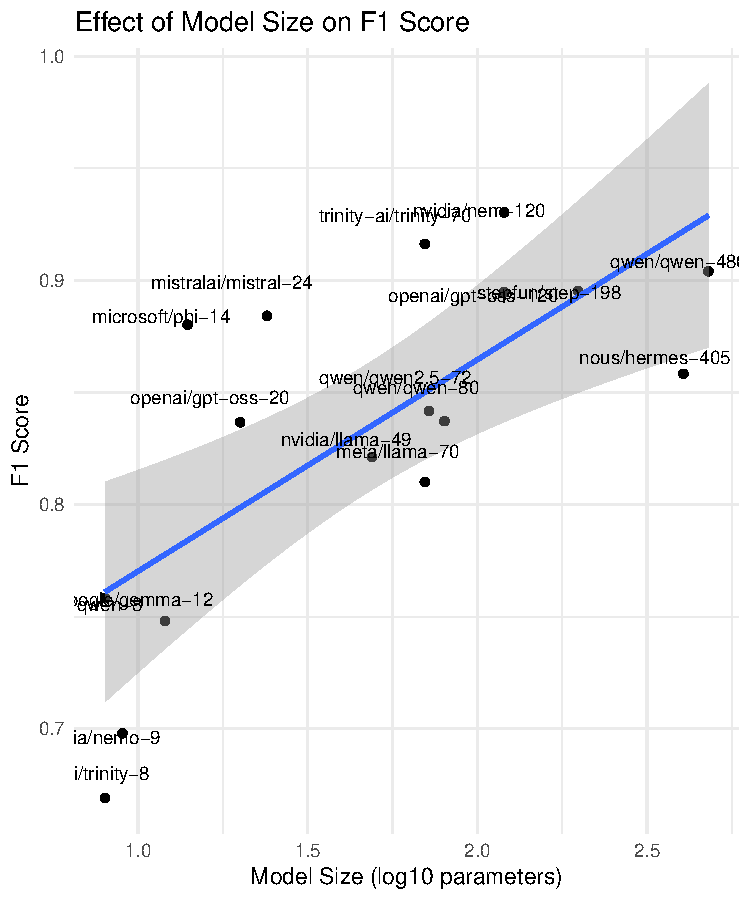
\includegraphics[width=0.95\columnwidth]{img/iRL-llm-fig-linear.pdf} 
\caption{F1 score vs. model size. The shaded band represents the 95\% confidence interval of the regression line.}\label{fig:linear}
\end{figure}

\begin{figure}[th]
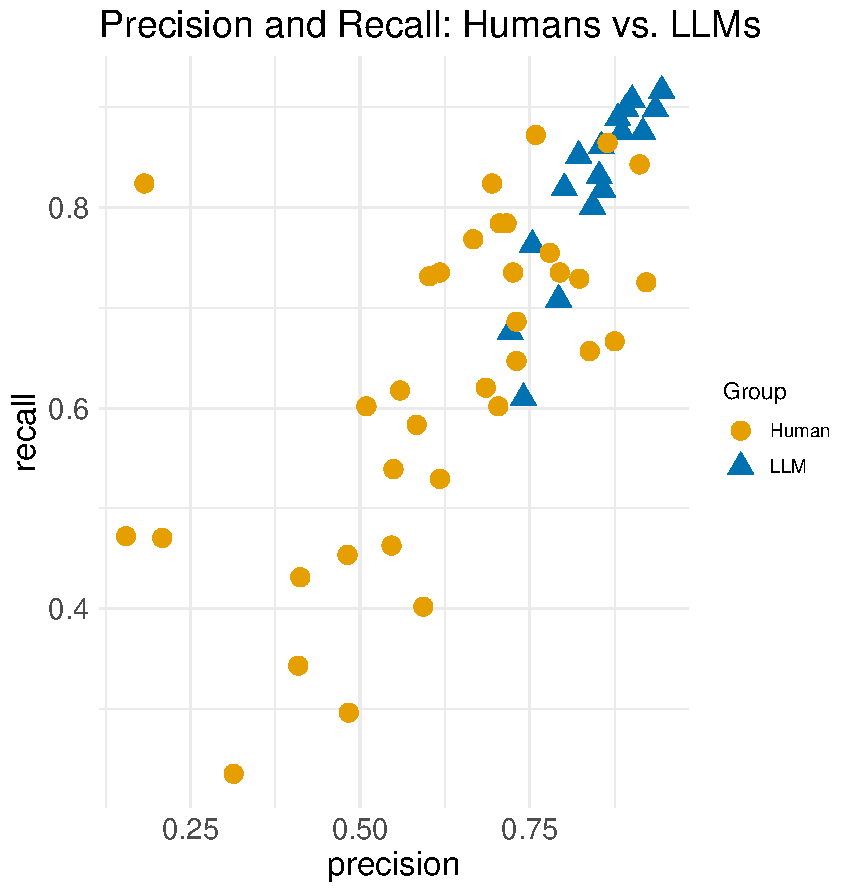
\includegraphics[width=0.85\columnwidth]{img/iRL-fig-scatter.pdf} 
\caption{Human vs. LLM performance}\label{fig:scatter}
\end{figure}



